\documentclass[12pt,a4paper]{article}
\usepackage[utf8]{vietnam}
\usepackage{amsmath}
\usepackage{amsfonts}
\usepackage{amssymb}
\usepackage{array}
\usepackage[left=2cm,right=2cm,top=2cm,bottom=2cm]{geometry}
\author{Huu Tai}
\usepackage{indentfirst}
\usepackage{footnote}
\usepackage{graphicx}
\begin{document}
\section{Giới thiệu}
Trong thời kỳ ngày càng phát triển của mạng internet thì việc chấm điểm tự động cho các bài tập lập trình ngày càng trở nên quan trọng hơn đặc biệt là khi có sự xuất hiện của các khóa học trực tuyến ngày càng phổ biến hoặc là các lớp học có sinh viên tham gia với số lượng lớn. Đánh giá là một phần không thể thiếu trong giáo dục và thường được sử dụng để đánh giá và cung cấp kết quả cho sinh viên tham gia vào môn học. Đồng thời dựa vào các kết quả đánh giá sau môn học của sinh viên mà giáo viên có thể xác định liệu chương trình giảng dạy có đáp ứng được nhu cầu cần thiết của sinh viên hay không.\newline  
\indent Trong lĩnh vưc giáo dục tâm lý, người ta đã chứng minh rằng hầu hết sinh viên thường hướng những nỗ lực của họ dựa trên kết quả của các bài kiểm tra sau khi được đánh giá và ảnh hưởng của các kết quả đó đến kết quả cuối cùng của khóa học. Tuy nhiên việc đánh giá kết quả một cách thủ công cho một lớp học đòi hỏi rất nhiều công sức và rất dễ bị lỗi và việc đấy càng được thể hiện rõ ràng khi số lượng sinh viên trong một lớp học tăng lên. Lúc đó việc đánh giá kết quả của sinh viên đòi hỏi phải được giới hạn hoặc hợp lý hóa theo một cách nào đó.\newline
\indent Trong thực tế hai giáo viên chấm cùng một môn rất hiếm khi áp dụng cùng một tiêu chí đánh giá trong mọi trường hợp. Điều này là không công bằng với sinh viên bởi vì điều đó có nghĩa là điểm đánh giá của học sinh có thể phụ thuộc vào từng giải pháp đánh giá của giáo viên mà không chỉ dựa vào giải pháp của học sinh. Và việc này càng xảy ra phổ biến trong việc đánh giá các bài tập lập trình.\newline
\indent Thông thường sẽ có vô số giải pháp khả thi cho cùng một vấn đề vì có thể có thể có các biến thể trong các lập trình do đó một mẫu đánh giá sẽ cũng cấp hướng dẫn cho người đánh giá nhưng sẽ không bao quát hết tất các cả trường hợp. Điều đó đòi hỏi phải có một công cụ giúp đánh giá các bài kiểm tra một cách tự động và hơn hết là đảm bảo đánh giá một cách công bằng, khách quan và được áp dụng như nhau cho tất cả học sinh.\newline
\indent Thách thức này đã dẫn đến sự phát triển của các công cụ chấm điểm tự động. Trong bài báo cáo này sẽ trình bày và so sánh các công cụ được sử dụng để chấm điểm tự động cho các bài tập lập trình.\newline
\section{Các lỗi phần mềm}
Trước khi trình bày về các kỹ thuật và hệ thống tự động đánh giá tôi muốn giới thiệu các lỗi thường được xem xét đến bởi các kỹ thuật này. Lỗi phần mềm được định nghĩa là tạo ra kết quả sai hoặc thực hiện một hành động theo cách không lường trước được. Lỗi phần mềm được phân loại thành các lỗi như: Lỗi cú pháp, lỗi logic và lỗi thời gian chạy.\newline
\subsection{Lỗi cú pháp}
Lỗi này được phát hiện khi cú pháp không chính xác trong ngôn ngữ lập trình, ví dụ như cấu trúc chương trình không chính xác, các từ sai, thiếu dấu chấm phẩy. Loại lỗi này có thể được trình biên dịch ngôn ngữ lập trình phát hiện trong khi biên dịch mã phần mềm. Lỗi này là lỗi dễ phát hiện và sửa nhất vì hầu hết các trình biên dịch được sử dụng ngày nay.\newline
\subsection{Lỗi logic}
Khi mắc lỗi này phần mềm biên dịch vẫn chạy tốt nhưng đầu ra của phần mềm bị sai do nhiều lý do như sai về yêu cầu hoặc đặc tả, lỗi toán học (chia cho 0). Vì lỗi này không được trình biên dịch phát hiện nên ta cần phát hiện các lỗi này trước khi khởi chạy phần mềm.\newline
\subsection{Lỗi thời gian chạy}
Đây là lỗi nâng cao và rất hiếm khi sinh viên bị rơi vào. Lỗi thời gian chạy chỉ xảy ra khi phần mềm đang chạy. Trong thực tế đây là một trong những vấn đề phức tạp nhất để theo dõi và dẫn đến sự cố phần mềm.\newline
\section{Lợi ích của việc sử dụng đánh giá tự động}
Việc áp dụng các hệ thống tự động đánh giá vào trong các khóa học đem lại các lợi ích sau:
\begin{itemize}
\item[-] \textbf{Tốc độ}: Giúp cho việc đánh giá nhanh hơn nhiều và sinh viên sẽ nhận được kết quả ngay sau kỳ thi. Khi sử dụng đánh giá thủ công thì sinh viên cần chờ một khoảng thời gian rất lâu để nhận được kết quả đánh giá của bài kiểm tra. Ngược lại với hệ thống đánh giá tự động, các sinh viên có thể tự đánh giá bài kiểm tra của mình, biết điểm của họ và sửa lỗi của chính họ.
\item[-] \textbf{Công bằng}: Các lỗi tương tự sẽ được đánh giá như nhau và giáo viên sẽ không ảnh hưởng đến việc chấm điểm.
\item[-] \textbf{Độc lập}: Việc đánh giá một bài kiểm tra không bị ảnh hưởng từ kết quả của các bài kiểm tra trước đó. Trong đánh giá thủ công, một bài kiểm tra lúc trước có kết quả không tốt có thê khiến giá viên chủ quan coi bài kiểm tra tiếp theo là không tốt.
\end{itemize}
\section{Các kỹ thuật được sử dụng trong đánh giá tự động}
\begin{itemize}
\item[-] \textbf{Unit testing}: Mục tiêu chính của bất kỳ phương pháp kiểm thử phần mềm là kiểm tra phần mềm đó có lỗi hay không, có tạo ra kết quả đầu ra đúng không và có tuân theo các thông số kỹ thuật được thực hiện bởi người kiểm thử phần mềm hay không. Unit testing đã đạt được sự nổi bật trong lĩnh vực khoa học máy tính và đó là một trong những phương pháp phổ biến nhất được sử dụng hiện nay để kiểm tra các đơn vị hoặc tính năng của phần mềm. Trong Unit testing, phần mềm được yêu cầu phải không bị lỗi cú pháp. Đầu ra của Unit testing cung cấp câu trả lời đúng hay sai. Người kiểm thử có trách nhiệm chuẩn bị các test case để thử nghiệm bao phủ tất cả các khía cạnh của đơn vị hoặc chức năng cần kiểm thử.
\item[-] \textbf{Sketching Synthesis  and Error Statistical Modeling (ESM)}: Là một công cụ để cung cấp phản hồi tức thì cho các bài tập lập trình. Ý tưởng chính đằng sau phương pháp này là cung cấp cho hệ thống một triển khai tham chiếu cho một vấn đề tính toán đơn giản như là ‘compute derivatives’. Công cụ này còn các hạn chế như: không kiểm tra các yêu cầu cấu trúc, không chấp nhận giá trị lớn, không hỗ trợ OOP.
\item[-] \textbf{Peer-To-Peer Feedback}: Phương pháp này người hướng dẫn làm cho sinh viên xếp loại ngẫu nhiên các câu trả lời khác nhau. Cách tiếp cận này có giúp cho sinh viên làm quen với các nguyên nhân lỗi, nhưng có các vấn đề gặp phải trong các hệ thống sử dụng phương pháp này như không có phản hồi cá thể làm cho sinh viên có thể đợi trong thời gian dài để nhận phản hồi và phản hồi sai hoặc không đầy đủ do kiến thức của sinh viên còn hạn chế.
\item[-] \textbf{Random Inputs Test Cases}: Phương pháp này đòi hỏi người hướng dẫn chuẩn bị một bộ đầu vào độc lập được sử dụng để kiểm tra đầu ra bài tập của sinh viên là đúng hay sai. Tuy nhiên khi sử dụng phương pháp này thì sinh viên sẽ không nhận được bất kỳ phản hồi nào cho thấy lỗi của sinh viên. Mục tiêu của bài kiểm tra này là kiểm tra xem sinh viên đã xác định đầu ra chính xác hay chưa vì vậy đối với phương pháp này sinh viên sẽ chỉ có 2 kết quả là đúng hoặc sai.
\item[-] \textbf{Pattern Matching}: Phương pháp này, người hướng dẫn cung cấp một đặc tả đầu của đầu ra rằng một phép gán đúng sẽ được giả sử để tạo ra và hệ thống yêu cầu các các công cụ Unix Lẽ và Yacc để tạo một chương trình xác minh rằng đầu ra từ các giải pháp của sinh viên gửi lên. Kỹ thuật này có nhiều nhước điểm vì nó chỉ chấp nhận và đưa ra một mức độ cho các giải pháp phù hợp hoàn hảo. Giáo viên hướng dẫn không thể phá vỡ mô hình để phân phối điểm trên các phương thức.
\end{itemize}
\begin{table}[ht]
	\centering
\begin{tabular}{|m{2.5cm}||m{2.5cm}||m{2.5cm}||m{2.5cm}||m{2.5cm}||m{2.5cm}|}
\hline 
Tool and Techniques & Sketching synthesis and error statistical modeling & Peer-to-peer feedback & Random input test cases & Pattern Matching & Unit testing\\ 
\hline 
Execution time & Nhanh (dưới 10 giây trong nhiều trường hợp) & Trung bình từ 40-60 giây & Chậm, mất nhiều giờ trong nhiều trường hợp & Nhanh (dưới 10 giây trong nhiều trường hợp) & Trung bình mất 30 giây\\ 
\hline 
Reliability & Chính xác (phụ thuộc vào test case được viết) & Có thể phát hiện 64\% lỗi & Không đáng tin cậy, nó phụ thuộc vào kiến thức của sinh viên & Trong một vài trường hợp (nếu tất cả đầu vào được bao phủ) & Trong một vài trường hợp (nếu tất cả đầu ra được bao phủ)\\
\hline
Dependency Test & Được hỗ trợ & Được hỗ trợ & Được hỗ trợ & Không hỗ trợ & Không hỗ trợ\\
\hline
Instant Feedback & Có & Có & Không & Có & Có\\
\hline
Support Oop & Có & Không & Có & Không & Không\\
\hline
\end{tabular}
\caption{Bảng so sánh các công cụ và kỹ thuật dùng trong Grade Student’Java Assessments.}
\end{table}
\section{Symbolic execution}
\subsection{Giới thiệu}
Trong hoạt động kiểm thử phần mềm, các ca kiểm thử thường được tạo ra một cách thủ công, gây tốn kém về chi phí cũng như thời gian để hoàn thành công đoạn này. Thực thi tượng trưng (Symbolic execution) được biết đến là một kỹ thuật nổi tiếng với khả năng tự động sinh những bộ test case có độ bao phủ cao với các tiêu chí kiểm thử nhằm phát hiện những lỗi sâu trong các hệ thống phần mềm phức tạp.\newline
\indent Hiện nay có rất nhiều công cụ nền tảng phục vụ cho hoạt động kiểm thử phần mềm như JUnit cho ngôn ngữ Java, Nunit, VSUnit cho .NET để thực thi các ca kiểm thử ở mức đơn vị. Tuy nhiên các công cụ kiểm thử này không hỗ trợ việc sinh tự động các ca kiểm thử đơn vị. Viết các ca kiểm thử là một công việc nặng nhọc và tốn nhiều công sức. Có nhiều phương pháp khác nhau hỗ trợ việc sinh tự động các ca kiểm thử (Test case) giúp giảm chi phí và thời gian thực hiện đã được nghiên cứu và đưa ra như: Dựa trên mô hình (Model Checking), kiểm thử ngẫu nhiên (Random Testing [1]). Nhưng hạn chế của nó là kiểm tra cùng 1 hành vị thực thi của chương trình nhiều lần với những đầu vào khác nhau và chỉ có thể kiểm tra được một số trường hợp thực thi của chương trình. Thêm vào đó, kiểm thử ngẫu nhiên khó xác định được khi nào việc kiểm thử nên được dừng lại và nó không biết tại điểm nào không gian trạng thái đã được thám hiểm hết. Để xác định khi nào việc kiểm thử dừng lại thì hệ thống kiểm thử ngẫu nhiên được kết hợp với các tiêu chuẩn an toàn [3]. Để khắc phục những hạn chế của kiểm thử ngẫu nhiên, phương pháp thực thi tượng trưng xây dựng các ràng buộc trên các giá trị tượng trưng và giải các ràng buộc đó để sinh ra các giá trị đầu vào cho chương trình mà nó có thể bao phủ tất cả các dòng lệnh cũng như các nhánh thực thi của chương trình.\newline
\indent Ý tưởng của thực thi tượng trưng đã được đề xuất bởi King [Comm. ACM 1976], Clarke [IEEE TSE 1976] nhưng việc hiện thực ý tưởng mới chỉ được thực hiện trong những năm gần đây qua tiến bộ đáng kể trong lý thuyết giải các ràng buộc (Constrain satisfiability) [11] và các tiếp cận mở rộng thực thi tượng trưng động (Dynamic symbolic execution), một kỹ thuật kết hợp giữa các giá trị cụ thể và giá trị tương trưng cho các giá trị đầu vào.\newline
\subsection{Tổng quan về kỹ thuật thực thi tượng trưng}
Ý tưởng chính của Symbolic execution là thực thi chương trình với các giá trị tượng trưng (Symbolic value) thay vì các giá trị cụ thể (concrete value) của các tham số đầu vào. Kết quả là giá trị đầu ra được tính toán bởi chương trình và được biểu diễn bởi bởi một biểu thức tượng trưng. Trong kiểm thử phần mềm, kỹ thuật Symbolic execution được sử dụng để sinh dữ liệu kiểm thử cho mỗi đường thực thi khác nhau của chương trình. Ví dụ trong hình 1 minh họa Symbolic execution.\newline
\indent Trong quá trình thực thi tượng trưng, việc đi theo một nhánh cụ thể nào đó không phụ thuộc vào các giá trị của các tham số đầu vào. Tại tất cả các điểm rẽ nhánh, tất cả các nhánh sẽ được xem xét và kiểm tra nhằm định hướng cho thực thi tiếp theo của chương trình. Với những chương trình ở dạng đơn giản có hại loại thực thi chủ yếu: đó là câu lệnh gán và câu lệnh rẽ nhánh. Tại các câu lệnh gán, giá trị tượng trưng của biến chương trình cũng như các tham số đầu vào có liên quan đến câu lệnh đó được tính toán và cập nhập lại, còn tại các điểm rẽ nhánh, chương trình sẽ điều khiển thực thi theo cả hai nhánh tương ứng đồng thời ràng buộc đường đi (Path condition) tương ứng với hai nhánh sẽ được tạo ra. Một ràng buộc là một biểu thức điều kiện tương ứng với giá trị true, ràng buộc kia tương ứng với giá trị false của biểu thức ràng buộc. Các ràng buộc này sẽ được cập nhập vào đường đi tương ứng với nhánh đó. Các ràng buộc này sẽ được xen xét bởi một bộ giải ràng buộc để đánh giá xem đường đi tiếp theo có khả thi không hay nói một cách khác là kiểm tra xem có tồn tại bộ giá trị thõa mãn ràng buộc này hay không. Nếu không thõa màn thì ràng buộc sẽ đánh giá là sai, khi đó Symbolic execution sẽ dừng hoặc quay lui thực thi theo nhánh khả thi.\newline
\begin{figure}[ht]
\begin{center}
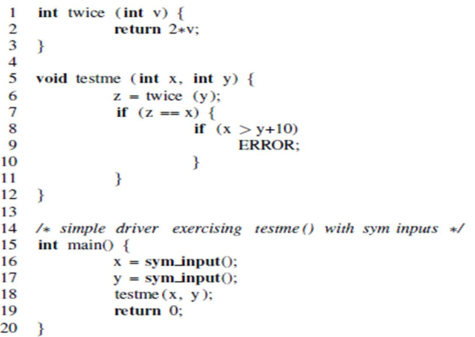
\includegraphics{hinhanh/hinh1}
\end{center}
\caption{Ví dụ cho symbolic execution}
\end{figure}
\indent Các ràng buộc đường đi được tạo ra bằng cách thu gom các điều kiện trên đường đi tương ứng. Giải các ràng buộc này sẽ sinh ra các giá trị cụ thể cho các tham số đầu vào tương ứng với từng nhánh thực thi của chương trình.\newline
\indent Tất cả các đường thực thi của chương trình có thể biểu diễn bởi một cấu trúc cây gọi là cây thực thi (Tree execution). Hình 2 là cây thực thi tượng trưng cho hàm testme() trong hình 1. Các cạnh của cây biểu diễn cho sự chuyển đổi từ trạng thái này sang trạng thái khác. Với ví dụ trên phương thức testme() trong hình 1 sẽ có cây thực thi mô tả những đường thực thi của chương trình với các biến đầu vào là {x=0, y=1}, {x=2, y=1}, {x=30, y=15}, mục tiêu là sinh ra tập các ca kiểm thử thõa mãn thực thi cho tất cả các nhánh của chương trình phụ thuộc vào giá trị tượng trưng của các tham biến đầu vào nhiều nhất có thể trong một khoảng thời gian nhất định đảm báo khám phá chính xác tất cả các đường thực thi bởi một lần duy nhất với những giá trị đầu vào đã cho.\newline
\begin{figure}[ht]
\begin{center}
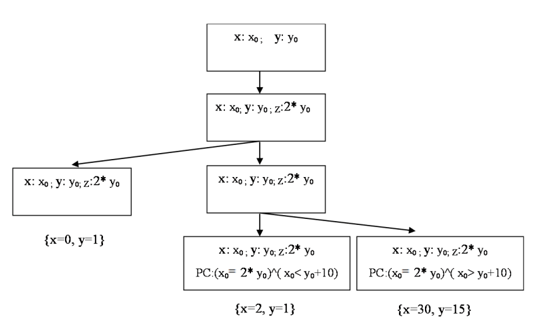
\includegraphics{hinhanh/hinh2}
\end{center}
\caption{Cây Symbolic execution tương ứng với hàm testme() trong ví dụ 1}
\end{figure}
\indent Bắt đầu thực thi tượng trưng hàm testme() bằng việc gán giá trị cho các tham số đầu vào x và y lần lượt là $x_0$, $y_0$. Khởi tạo PC (Path condition) nhận giá trị là true, tới câu lệnh rẽ nhánh $if(2*y_0=x_0)$ hai nhanh của chương trình tương ứng đều được thực thi với các giá trị tương ứng là $x_0$ và $y_0$. Tại đây biểu thức điều kiện rẽ nhánh là $2*y_0=x_0$ và $!(2*y_0=x_0)$ được bổ sung và PC theo hai nhánh khác nhau. Sau khi thực thi câu lệnh $if(2*y_0=x_0)$ hàm testme() được thực thi theo nhánh mà tồn tại bộ giá trị x,y thõa mãn. Tương tự như trên, khi gặp câu lệnh $if(x_0>y_0+10)$ PC theo hai nhánh tương ứng sẽ được cập nhập bổ sung là $(2*y_0=x_0)$ \^{} $(x_0>y_0+10)$ và $(2*y_0=x_0)$\^{}$(x_0<y_0+10)$. Tại mỗi điểm rẽ nhánh PC sẽ được cập nhập và một thủ tục quyết định bằng bộ xử lý ràng buộc sẽ được sử dụng để xác định xem nhánh tương ứng với PC đó có khả thi hay không để điều hướng thực thi hiện thời đi theo nhánh đó. Nếu PC được đánh giá là không khả thi thực thi tượng trưng sẽ dừng hoặc quay lui, và thực thi tượng trưng chỉ thực thi chương trình tượng trưng theo nhánh mà PC được đánh giá là khả thi.\newline
\indent Đối với những đoạn mã chứa vòng lặp hoặc lời gọi đệ quy mà đường thực thi là vô hạn và biến điều khiển của vòng lặp hoặc lời gọi đệ quy là tượng trưng. Ví dụ trong hình 3 sẽ là vô hạn đường thực thi với mỗi đường thực thi là 1 dãy tùy ý số lượng giá trị là true và sau cùng là false hoặc là một dãy vô hạn số lần lặp, khi đó PC của đường thực thị là một dãy gồm n giá trị true và sau cùng là false.\newline
\begin{figure}[ht]
\begin{center}
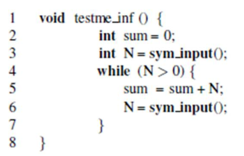
\includegraphics{hinhanh/hinh3}
\end{center}
\caption{Ví dụ cho vòng lặp vô hạn}
\end{figure}
\indent Trên thực tế cần phải thêm các tiêu chí giới hạn cho việc tìm kiếm như thời gian thực thi, giới hạn chiều sâu của đường thực thi hoặc số lượng các vòng lặp lồng nhau.\newline
\indent Nhược điểm chính của Symbolic execution truyền thống là không thể sinh dữ liệu test nếu không giải được biểu thức ràng buộc đường thực thi. Ví dụ nếu ta thay hàm twice() ở hình 1 bằng hàm twice() ở hình 4 sau khi thực hiện câu lệnh dòng 7 thì thực thi tượng trưng sẽ cho ra hai ràng buộc mới bổ sung $x_0$\#$y_0$*$y_0$\%50 và $x_0=y_0$*$y_0$\%$50$ và khi bộ giải ràng buộc không giải được ràng buộc trên thực thi tượng trưng sẽ thất bại trong việc sinh các dữ liệu kiểm thử cho chương trình sau khi đã được sửa đổi.\newline
\begin{figure}[ht]
\begin{center}
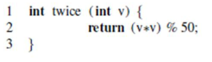
\includegraphics{hinhanh/hinh4}
\end{center}
\caption{Ví dụ cho hàm twice()}
\end{figure}
\end{document}
